\documentclass[12pt]{article}

\usepackage{sbc-template}
\usepackage{graphicx,url}
\usepackage[round, numbers]{natbib}


%\usepackage[brazil]{babel}   
\usepackage[utf8]{inputenc}  

     
\sloppy

\title{Gamified Language Learning: Enhancing Learning through Streaming Services and SRS}

\author{J. Emanuel Cascone R. S.\inst{1}, Guilherme A. Avelino\inst{1} }


\address{Computer Science Department - Federal University of Piauí (UFPI)\\
  Teresina, PI -- Brazil
  \email{\{emanuelcascone,gaa\}@ufpi.com.br}
}  
\begin{document} 

\maketitle

\begin{abstract} 
 The process of learning a new language typically commences with activities such as writing, reading, listening, and speaking. This work involved creating an application that facilitates language learning by utilizing a movie streaming platform with subtitles, allowing users to watch movies with the original audio and subtitles and focus on keywords or frequently repeated words for better comprehension. The work is based on the premise that to understand a text, you don't necessarily need to know the whole formation but rather just the keywords or most repeated words, allowing you to apply skimming and scanning techniques. To record these words in the user's memory, gamified forms of Spaced Repetition System (SRS) can be applied to induce the user to better adapt to each scenario in the future based on their current repertoire. By following this approach, users can enhance their experience while watching movies or videos to acquire knowledge of a new language. \\
  \textbf{Key words:} language learning, gamification, streaming platforms, subtitles, SRS, skimming, scanning
\end{abstract} 


\section{Introduction}
Mastering a new language is undeniably valuable, yet it's often accompanied by challenges such as waning motivation and a sense of discomfort. What if there was a way to transform language acquisition into an engaging and less taxing experience? Imagine users effortlessly learning while enjoying themselves. \\
In parallel, watching movies and series has become a widespread and enjoyable activity, with streaming platforms emerging as a popular source of entertainment. Incorporating bilingual subtitling into these platforms, as explored by \cite{Gouleti-Katerina}, offers a promising avenue. This mode of audiovisual translation not only enhances accessibility but also serves as a potent pedagogical tool for language learners. The integration of bilingual subtitles in streaming media aligns with the evolving preferences of digital natives, facilitating active engagement and effective language acquisition strategies.\\
\cite{Birules-Muntane2016-on} conducted a study demonstrating that watching subtitled films improves speech perception skills significantly, particularly when viewers engage with the original language and corresponding subtitles. Their findings underscore how subtitled media, even in relatively short exposures, can foster perceptual learning crucial for language acquisition, thus supporting the notion that multimedia engagement enhances language learning outcomes.
By leveraging such technological innovations, this approach aims to make language learning more intuitive and enjoyable, addressing the shortcomings of traditional methods and fostering sustained motivation among learners.
Studies demonstrate that students acquire a new language at double the speed using a similar learning mechanism called smart subtitles \cite{Kovacs13}. The fusion of these concepts (entertainment and study) has the potential to help language learning, making it more engaging and less taxing. \\
This work is about the creation of an application that allows users to learn a new language or expand their vocabulary in a gamified and interactive manner using streaming platforms.
Creating new alternatives to make learning a new language more exciting and efficient is the motivation for this work. Because the conventional language learning method can be tiresome and demotivating for many students. \\
By creating an environment that allows interaction with streaming sites for movies, learning a new language can be done more naturally and playfully, similar to tools that translate web pages to facilitate learning or understanding of other languages already present in the market or research area \cite{ElBatanony21}. \\
Watching movies with audio and subtitles in the original language, the user can learn while applying gamified Spaced Repetition System (SRS) techniques to memorize new words. In succinct terms, the motivation for this work is to provide an efficient and attractive alternative for learning new languages.
The traditional method of learning a new language can be exhausting and demotivating for many students. A more playful and interactive approach to learning new languages is necessary to make the process more enjoyable and efficient. \\
The work is based on the premise that learning a new language more efficiently and satisfactorily is possible when gamified and interactive. Additionally, it is based on a similar methodology - smart subtitles - which has been effective in expanding vocabulary \cite{Kovacs14}. \\
Thus, the goal is to offer a different and efficient approach to using subtitles so that people can learn new languages and expand their vocabulary while watching their favorite movies in a relaxed and effective way.\\
The rest of the paper is structured as follows: Section 2 presents the methodology used in the study. Section 3 provides a theoretical referential, discussing the concepts and theories that underpin the work. Section 4 delves into the software design, detailing the architecture and components of the application. Section 5 presents the results of the study, including the MVP and user feedback. Finally, Section 6 concludes the paper, summarizing the key findings and outlining future directions for the research.



\section{Methodology}
This study employed a two-phased methodology to achieve its objectives. The first phase encompassed a comprehensive review of existing research and theoretical frameworks relevant to the gamification of language learning. This review examined prior work and theoretical foundations related to two key areas:

\begin{enumerate}
    \item \textbf{Strategies and technologies for promoting playful and interactive language acquisition}: This included investigating successful implementations of gamification in educational contexts and analyzing their impact on learner engagement and knowledge retention.
    \item \textbf{User training methodologies for optimizing progress in digital learning environments}: This involved exploring best practices for onboarding users, providing effective guidance and feedback, and leveraging user data (such as learning progress and preferences) to personalize the learning experience and enhance its efficacy.
\end{enumerate}

 

Building upon the insights gleaned from this comprehensive review, the second phase focused on the development of a functional prototype. This prototype served as a platform for preliminary testing and evaluation of the proposed gamified language learning approach, with a particular emphasis on user experience. 


\section{Theoretical Referential}
In recent years, there has been a growing interest in the use of subtitled videos as a way to assist in the learning of foreign languages. However, standard subtitles are not ideal for vocabulary acquisition, as translations are non-literal and are provided only for phrases, not individual words. \\
To overcome this problem, "Smart Subtitles" have been developed, interactive subtitles focused on vocabulary acquisition. "Smart Subtitles" includes features such as vocabulary definitions when hovering over with the mouse cursor and video navigation based on dialogue \cite{Kovacs13}. Studies have shown that students learn more than double the vocabulary with "Smart Subtitles" compared to Chinese-English dual subtitles, with similar levels of comprehension and satisfaction \cite{Kovacs14}. \\ he learning of foreign languages is the use of browser extensions. The browser extension "InteractiveSubtitle" \cite{ElBatanony21} is an example of this. The extension features personalized learning, translation of phrases in context on web pages, and support for over 100 languages. The goal is to utilize various hypotheses of foreign language acquisition to create a new language learning tool that is more effective. \\ 
Some students of languages don't adopt this method but adopt methods such as SRS, which is a technique tested and proved effective by Landauer and Bjork in 1978, that involves reviewing information at increasing intervals. This technique is used in apps like Anki, Duolingo, and others, and is a technique that is used to improve the user experience and learning outcomes. \\
Based on these ideas, an application has been proposed that utilizes a real kind of "Smart Subtitles" to train users through gamified practice before watching a subtitled movie in a language they are learning.   \\
\subsection{Subtitles}
Smart subtitles and dual subtitles have emerged as innovative solutions to enhance the multilingual viewing experience for audiences worldwide. These technologies leverage advancements in natural language processing and multimedia to provide seamless translation and accessibility options for viewers. \\
Dual subtitles offer a unique viewing experience by presenting multiple languages simultaneously on-screen. This method is particularly beneficial for language learners and bilingual audiences seeking to improve their language proficiency. The concept of dual subtitles has been explored by scholars such as Dr. François Yvon, who has investigated its effectiveness in language acquisition and comprehension.\\
Studies conducted by researchers such as Dr. Spela Vintar and Dr. Koen van Turnhout have demonstrated the effectiveness of smart subtitles and dual subtitles in improving language learning outcomes and comprehension rates. Their research highlights the potential of these technologies to bridge language barriers and promote cross-cultural understanding in multimedia contexts.\\

\subsection{Spaced Repetition System (SRS)}
Spaced Repetition Systems (SRS) have revolutionized the way we learn and retain information. The concept of spaced repetition dates back to the 19th century, but it gained significant attention and refinement in the digital era. This method leverages the psychological spacing effect, where information is better retained when revisited at increasing intervals over time. \\
One of the most influential implementations of SRS is \textit{SuperMemo}, developed by Dr. Piotr Wozniak in the late 1980s. SuperMemo was one of the first computer-based systems designed to optimize the learning process through spaced repetition algorithms. Wozniak's work has inspired numerous SRS applications and research studies worldwide.\\
Research conducted by cognitive psychologists such as Dr. Sebastian Leitner further validates the effectiveness of spaced repetition. Leitner introduced the \textit{Leitner system}, a practical implementation of spaced repetition using flashcards arranged in different boxes based on recall success. His work demonstrates how SRS can enhance long-term retention compared to traditional learning methods.\\

\section{Software Design}
The application core (the method of teaching) is based on the articles by Kovács et al. \cite{Kovacs14}, which use the premise of subtitles to advocate for a more playful and immersive learning method. This demonstrates the potential of such approaches for language learning and how more playful and intelligent approaches directly influence learning new words, as exemplified in Figure-\ref{fig:my_label}. 
\begin{figure}[!h]
\centering
\caption{Learning curves for new words using two types of subtitles and smart subtitles}
\label{fig:my_label}
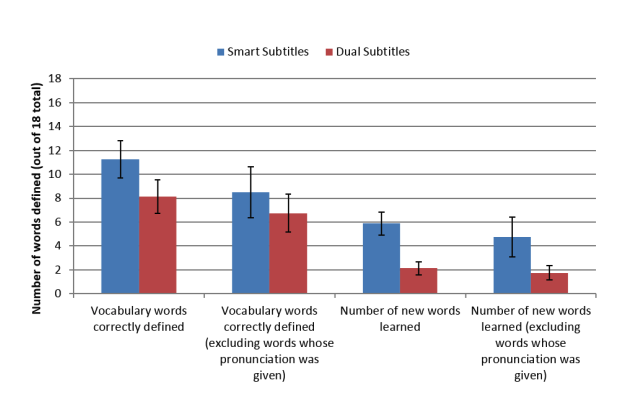
\includegraphics[width=0.7\textwidth]{assets/3.png}
\end{figure} 
\begin{figure}[!h]
  \centering
  \caption{
    Container Diagram for the application
  }
  \label{fig:container_diagram}
  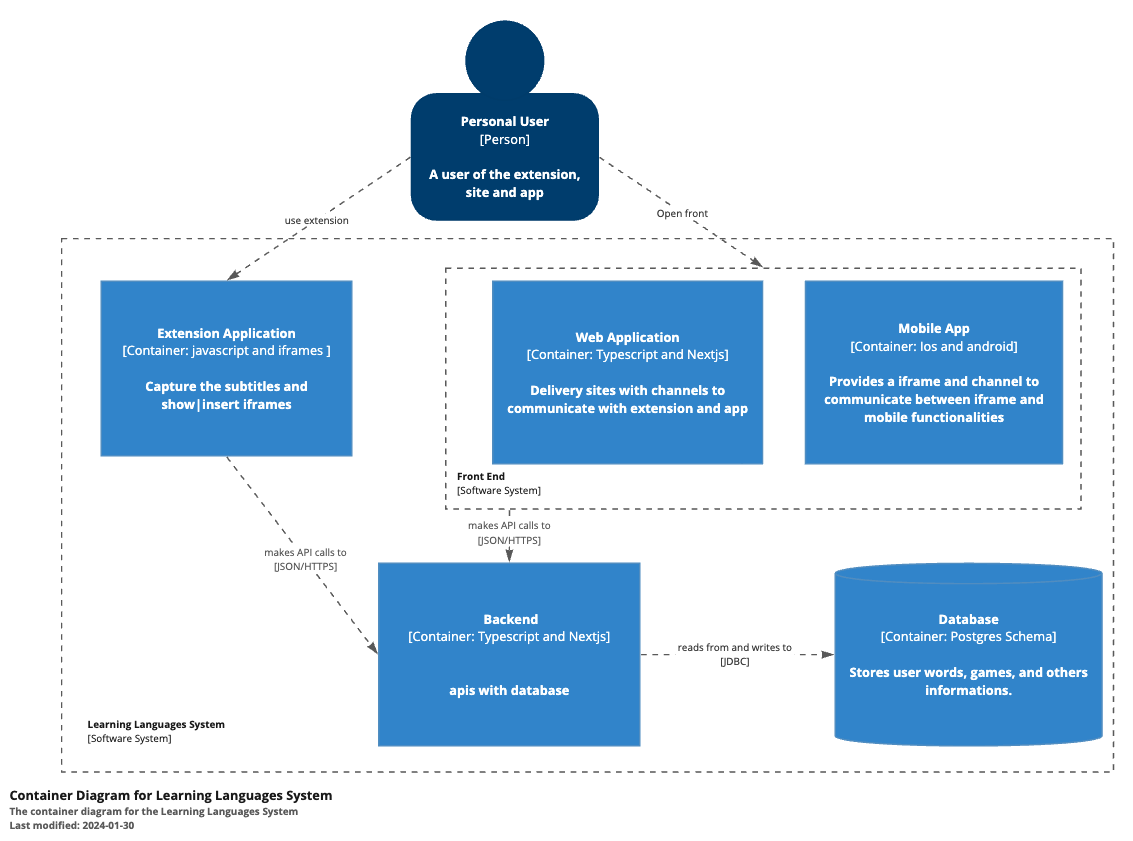
\includegraphics[width=0.9\textwidth]{assets/24.png}
\end{figure}
\begin{figure}[!h]
  \centering
  \caption{
    The flow of the application until the use of AI
  }
  \label{fig:flow_diagram}
  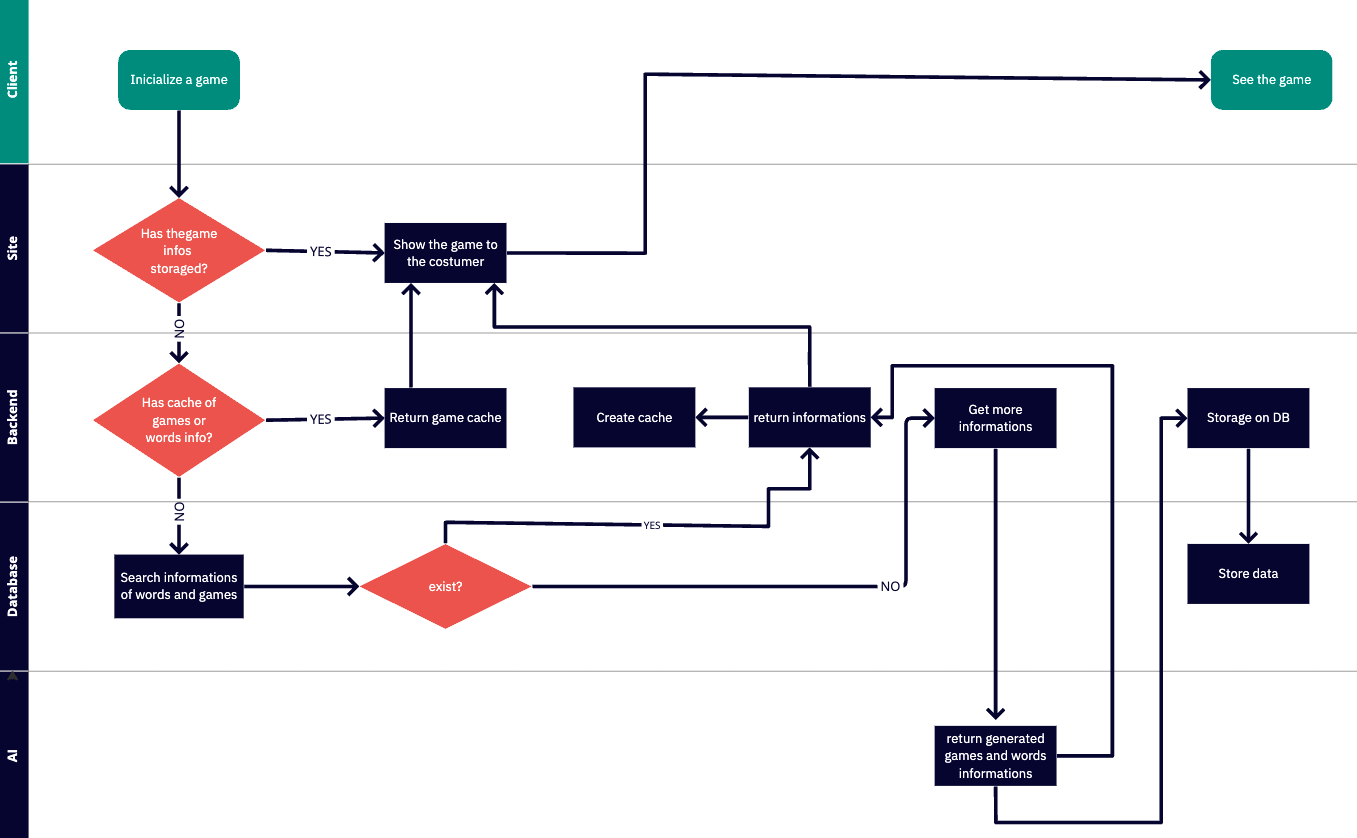
\includegraphics[width=0.9\textwidth]{assets/26.png}
\end{figure}
Using Spaced Repetition System (SRS) techniques to gamify learning new languages based on the premise that knowledge of keywords or the most repeated ones allows for text comprehension. \\
At this point in the prototype creation, an environment to learn a new language was built, including a browser extension, a site, and an app, all integrated and working together to provide a better experience. \\
The Container diagram, depicted in Figure-\ref{fig:container_diagram}, offers a detailed visualization of the application's architecture, delineating the interactions between different components such as the extension, site, and app. This diagram showcases the technological framework utilized and elucidates how these components collaborate to facilitate seamless communication and functionality. \\
The core of the system is an AI provided by openAI, to generate translations, meanings, and games. Each one of the environments has its functions and responsibilities. The extension is responsible for capturing the subtitles and opening the modal with the iframe, the site is responsible for storing the data and providing the games, and the app is responsible for showing the site inside the iframe and sending the user information to the site. \\
To be more visible the process of the games and word data acquisition, the figure-\ref{fig:flow_diagram} illustrates it. This flow was selected with a focus on optimizing speed due to the substantial volume of data involved, along with the associated costs of utilizing AI. \\
Presently, the AI of choice is the gpt-3.5-turbo-0125 model developed by OpenAI, incurring costs of input is \$0.50/1M tokens (the unit used in AI system) and output is  \$1.50 / 1M tokens. Leveraging a database for storing data offers greater flexibility, particularly since the input remains constant. This approach ensures that when a user learns a word in a specific language and transitions to another, the necessary information about games and the word parameter are retrieved from the AI only once. 
\subsection{Extract algorithm}
The filter algorithm is a critical component of the application, as it is responsible for identifying and extracting words from subtitles. For each platform (e.g., Prime Video, Netflix, Disney+), the algorithm must be tailored to the specific structure of the subtitles. \\
The algorithm is inserted into the extension and is responsible for capturing the subtitles and sending them to the site. \\
But the result is the same for all platforms, a JSON structure with the words, the moments where the words appear, and the count of the words, and the percentage of the word in the subtitle. \\
The algorithm runs a pipeline that takes the subtitle in TTML format converts it to JSON format, and then processes the JSON to extract the words and their respective counts, and phrases where the word exists, and determine the position and percentage of each word. 
\subsection{Artificial Intelligence}
  Artificial intelligence (AI) is a critical component of the application, as it is responsible for providing translations, meanings, and games. The AI receives a prompt based on the user's request, and the AI returns the requested information. 
  An example of the prompt is \\
  \begin{verbatim}
    I am a bot that generates quizzes for you to learn 
    new words. 
    My quiz is not very good at it, but I am learning.
    Help me to learn by generating a quiz.
    The quiz is a phrase using a word in the 
    language and you need to translate it to the 
    target language.
    The options are a list of words to choose the correct 
    translation for the word in the target language. 
    The options are made by others' translations of the 
    target language or translation of similar words.
    ```
    ...rest of the prompt contends an 
    example of input and output expected by the AI
    ```
  \end{verbatim}
  Currently, the prompt is used to generate the quiz, but AI is employed also to generate translations and meanings of the words. Once the AI receives the prompt and returns the requested information, the backend processes and stores it in the database. Storing the quiz is crucial because each request to the AI incurs a cost, which is determined by the number of tokens used in the request. \\
  If the approach were to manually create a database and quizzes, both the cost and time investment would significantly increase, leading to a deterioration in user experience. Given the large number of words required to generate a quiz, users would face a substantial learning curve in acquiring a new language.

\subsection{Games}
  The games are developed to transform the learning process singleton, which means that each word has its own line of learning and when appears on the user screen the user does something that answers if the user knows the word or not. \\
  Choose three games to generate, the first one is a quiz, the second one is a word search, and the third one is a flashcard. \\
  The quiz shows a phrase using a word in the language and the user needs to choose a correct translation for the word in the target language. The options are made by the AI. \\
  The word search is about showing a word in the language and the user needs to find the correct translation for the word in the target language. The options are made by the AI. \\
  The flashcard goal is a word in the language and the user needs to choose whether he knows the word or not. \\
  Those games are designed based on apps like Anki and Duolingo.
\subsection{Learning algorithm}
Based on SRS and the games generated by the information provided by the AI, as the games are designed to transform the learning process singleton when the API sends information about the word, the game will show based on priority specificated on the API. \\
More priority is that the word will appear on the user screen, and the user will see the word more often. \\
\begin{enumerate}
  \item Is today the day for learning?
  \item How often does it repeat? 
  \item Are there any errors?
\end{enumerate}
Following those questions, the server(API) ranks and filters the words. 
\subsubsection{Is today the day for learning?}
As the API uses an SRS technique, the API needs to know if today is the day for learning the word. The approach chosen was an exponential function, that is based on the number of times that the user saw the word and when the user made a mistake. The function is based on the following formula:
\begin{equation}
  \label{eq:1}
  f(x, y) = 2^x 
\end{equation}
Is a simple equation, for example: if the user sees the word today and doesn't make a mistake, he will see the word again in 2 days, if the user continues without making a mistake, he will see the word again in 4 days, and so on. But if the user makes a mistake, the function will be reset and the user will see the word again in 1 day. \\
That question filters the words that the user will see today. 
\subsubsection{How often does it repeat?}
The server also knows how common is this word (based on the entire database) and how common this word is on subtitles. The server gets the percentage of the word in the subtitle and the percentage of the word in the entire database, and based on that sort creates a ranking of the words. \\
Each of that information is 50\% of that ranking, and the server creates a ranking based on that information. 
\subsubsection{Are there any errors?}
The API also knows how many errors the user makes with that word, and how many errors the entire database makes with that word. The API gets the percentage of the word in the subtitle and the percentage of the word in the entire database, and based on that the server creates a ranking of the words. \\
As in the previous step, the server creates a ranking based on that information, taking 50\% of the database and 50\% of the user. \\




\section{Results}
A browser extension was developed that interacts with movie streaming sites and extracts the subtitles available on these sites. The extension uses Spaced Repetition System (SRS) techniques to gamify learning new languages based on the premise that knowledge of keywords or the most repeated ones allows for text comprehension. The goal is to expand to other platforms like Netflix, Disney+, and others. \\ 
The site was also developed to provide statistics on user progress, including the most challenging words, the total words learned, and others to help the user understand their learning process. The site also supports multiple languages, which allows users to learn a wide range of languages using AI translations and the creation of games.  \\
The app was developed to provide a way for the user to study on every device, displaying the iframe with the application site.\\
This work has demonstrated the potential of using technology to facilitate language learning. Integrating our tool with everyday activities such as watching movies can make language learning more engaging and compelling. 

\subsection{MVP}
The application was publicly released on the website and the extension was published on the Chrome Web Store. The application is available for users to download and use. The application is currently in the MVP stage, with basic features and functionality. The MVP includes the features previously mentioned. \\
The MVP is a prototype that demonstrates the potential of using technology to facilitate language learning. The MVP is a proof of concept that showcases the core functionality of the application. The MVP is a starting point for future development and improvements. \\
\begin{figure}[!h]
  \centering
  \caption{
  Cloud words of the reviews of the users
  }
  \label{fig:cloud_words}
  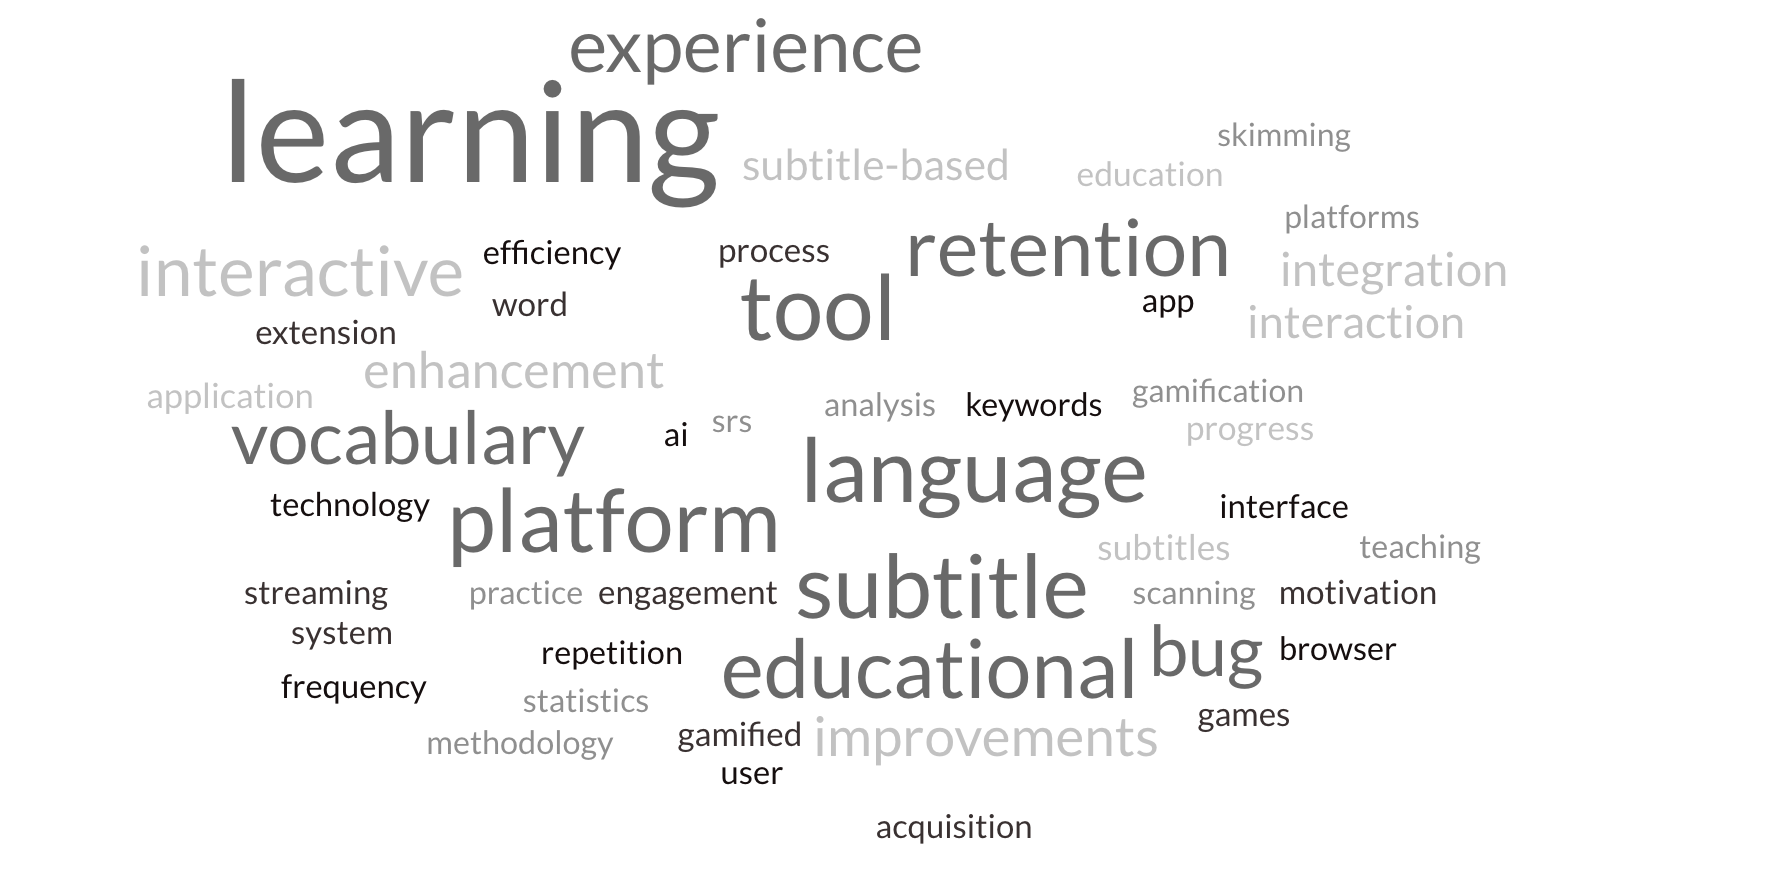
\includegraphics[width=0.7\textwidth]{assets/33.png}
\end{figure}
A control group has used the application after knowing how it work on the background and the methodology used to learn the words. The group has been asked to use the application and write a small review, where the keywords can be visualized in a cloud of words. The cloud words can be seen in the figure-\ref{fig:cloud_words}.

\begin{frame}{}
  \begin{figure}[!h]
      \begin{minipage}[b]{0.5\linewidth}
        \centering
        \caption{
        Database data of words, attempts, and movies
        }
        \label{fig:database_data}
        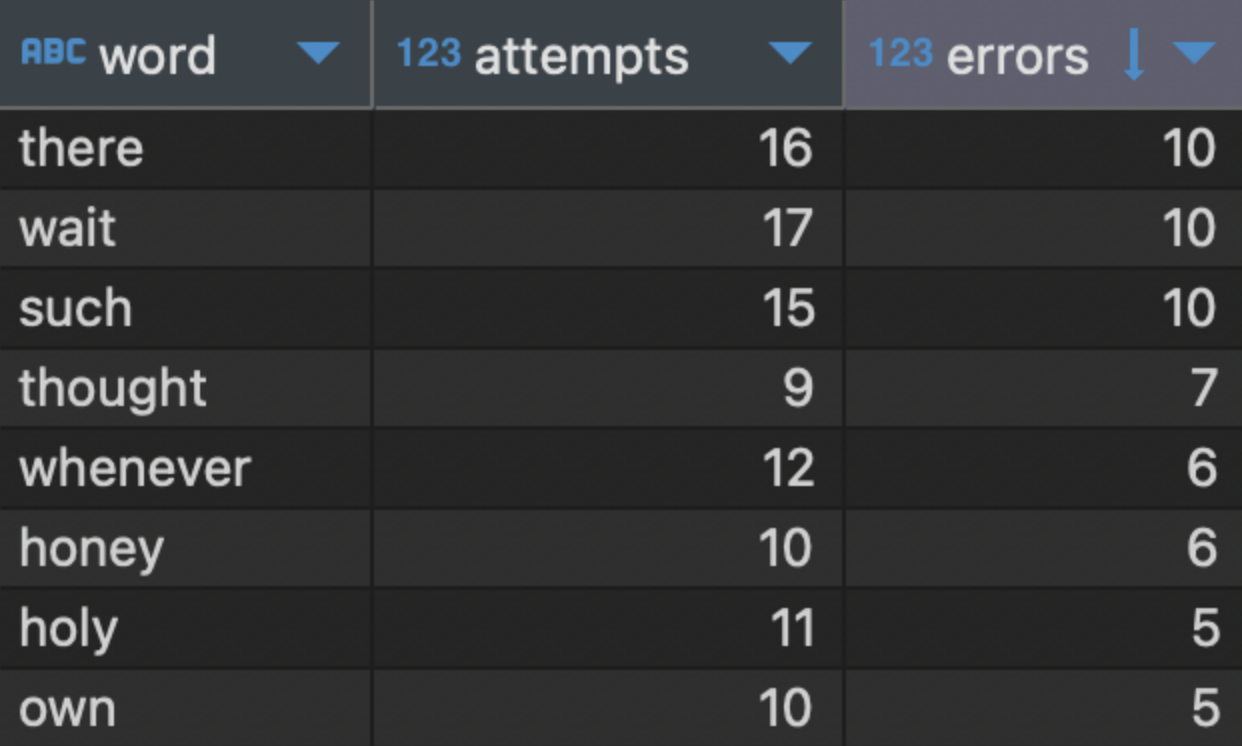
\includegraphics[width=1\textwidth]{assets/32.png}
      \end{minipage}
      \hspace{0.1cm}
      \begin{minipage}[b]{0.5\linewidth}

        \centering
        \caption{
        Words with the most errors
        }
        \label{fig:database_errors}
        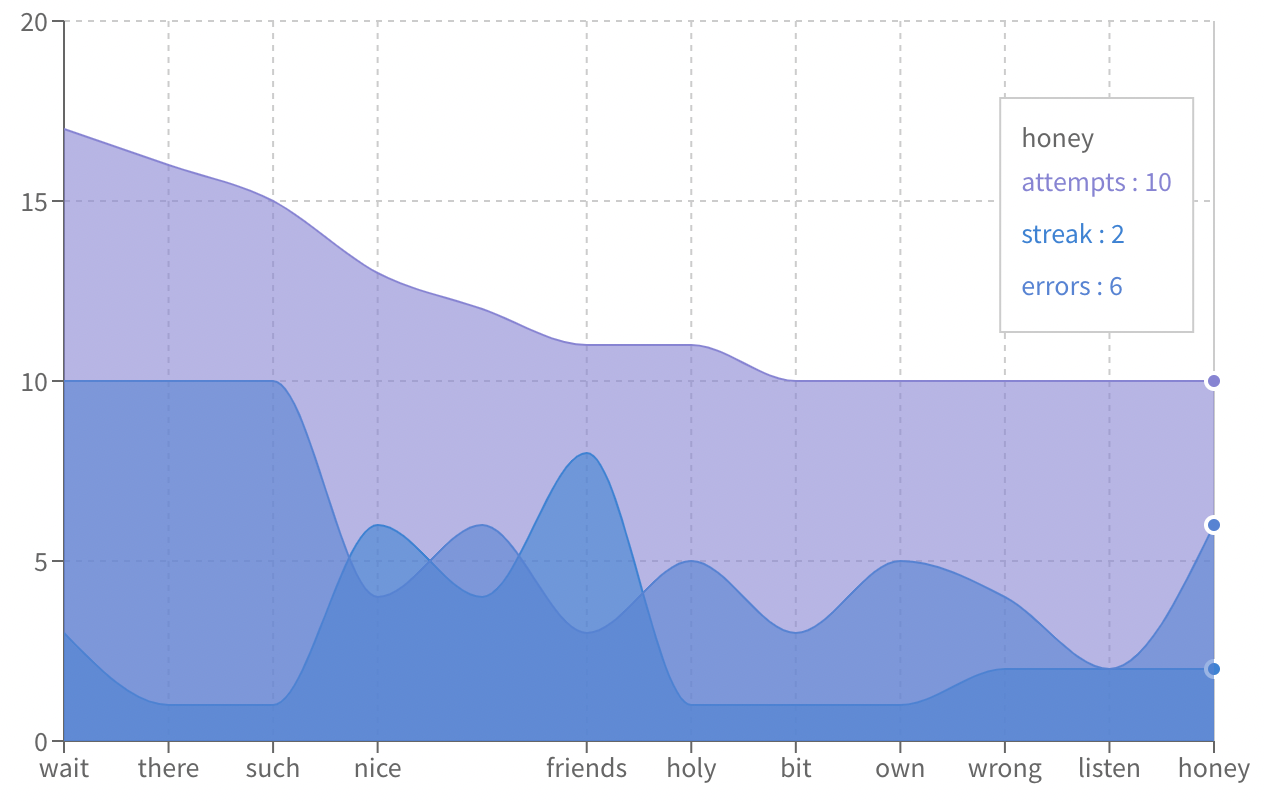
\includegraphics[width=1\textwidth]{assets/30.png}
       \end{minipage}
  \end{figure}
\end{frame}
The database provides information about the words, allowing the user to analyze the user's behavior and the words that the user is learning. The database has information about the words, the attempts, and the movies, as demonstrated in the figure-\ref{fig:database_data}. 
It's possible to see the words with the most errors, as demonstrated in the figure-\ref{fig:database_errors} (which contains the 12 words with the most errors in the database). The server will prioritize those words to appear on the user screen, and the user will see the word more often. 
\begin{figure}[!h]
  \centering
  \caption{
  Streaks, errors, and attempts of the users
  }
  \label{fig:database_users}
  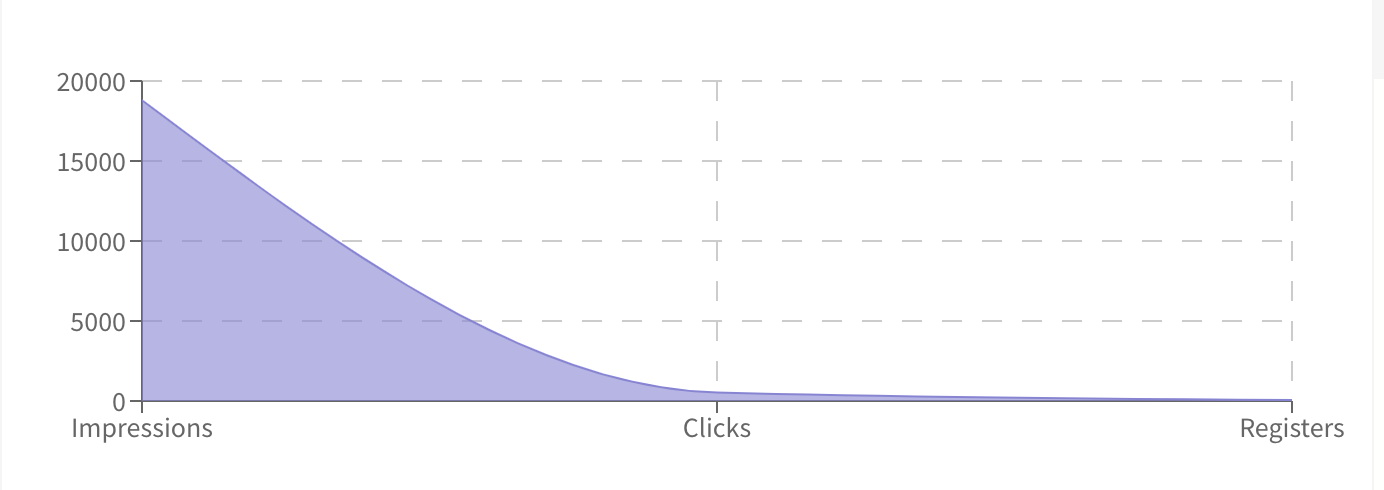
\includegraphics[width=0.50\textwidth]{assets/31.png}
\end{figure}
The server also knows the streaks, errors, and attempts of the users, as demonstrated in the figure-\ref{fig:database_users}. Some users have already tried to learn words 880 times. And is possible to analyze that 
most errors appear in the word, the more the users will train that word and the more attempts will have, as seen in the figure-\ref{fig:database_users}. \\
Until now the application has been well received by users, the database has been growing, and the application has been used by a significant number of users, 58 at the time of writing (16/06/2024). The tax of conversion follows that funnel of conversion, as demonstrated in the figure-\ref{fig:database_errors}. 
But it is also possible to see that the streaks (times that the user saw the word without making a mistake) are growing, and the users are learning the words, as demonstrated in the figure-\ref{fig:database_users}. \\
When the streak line is bigger than the error line, the user is learning the word, and the server will decrease the priority of that word to appear on the user screen. \\
During that period the users have tried to learn the words of 22 movies and a total of 1049 words. It means that each movie tries to learn as a media of 47 words. with a media of 5.58 attempts per word with more than 1 error. And a medium of 2.98 errors per word with more than 1. \\


\section{
Conclusion
}
This work has successfully developed a browser extension, a website, and an app that aims to facilitate language learning by extracting subtitles from movie streaming sites. The extension utilizes Spaced Repetition System (SRS) techniques to gamify language learning, while the website provides statistics on user progress and supports multiple languages. The app allows users to study on any device. \\
Moving forward, several steps are planned for each application component. The extension will be expanded to other streaming sites, languages, and platforms and it will be integrated with other language-learning tools. The website will include interactive exercises, games, and customized learning experiences. The app will capture device information and improve communication with the website. \\
In addition, the application's backend will be enhanced with improvements to API routers and to the language manager. Web sockets will improve communication between the extension and the website. \\
Overall, this work demonstrates the potential of using technology to make language learning more engaging and accessible. By integrating language learning with everyday activities like watching movies, users can enhance their language skills in a fun and interactive way.\\







\bibliographystyle{sbc}
\bibliography{sbc-template}
\hfill \\
\hfill \\
\hfill \\
\hfill \\
\hfill \\
\hfill \\
\hfill \\
\hfill 
\centering

\end{document}